\begin{highlightblock}[Task: Sequential circuit]
In this exercise a delay circuit should be programmed. After pressing the start
    button a counter is started and increments until it reaches its maximum
    value. If this value is reached the output led is activated and the counter
    is restarted from zero. If the counter reaches its maximum value again, the
    out- put led is deactivated and the system waits until the start button is
    pressed again. Figure \ref{fig:delay} shows the blocks which should be
    implemented to realize the delay circuit. The circuit contains a counter
    which is used to produce a delay

\begin{center}
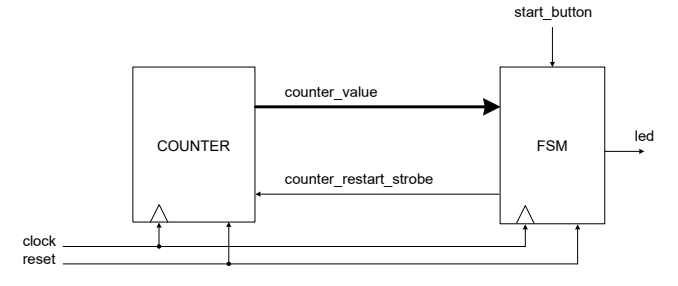
\includegraphics[width=0.8\linewidth]{images/Block.png}

Figure \refstepcounter{figure}\arabic{figure}: Block diagram of the delay circuit\label{fig:delay}
\end{center}

and a finite-state-machine (FSM) which controls the counter and the interaction
    with the start button and the led output. Furthermore the needed signals
    be- tween these two blocks can be seen in figure \ref{fig:delay}. The
    signal counter value holds the current counter value, counter restart
    strobe is used to reset the counter value to zero.

\end{highlightblock}

\begin{highlightblock}
Figure \ref{fig:fsm} shows the states and transitions of the used finite state
    machine. The edges are labeled with the events that must happen for a
    transition into the next state.

\begin{center}
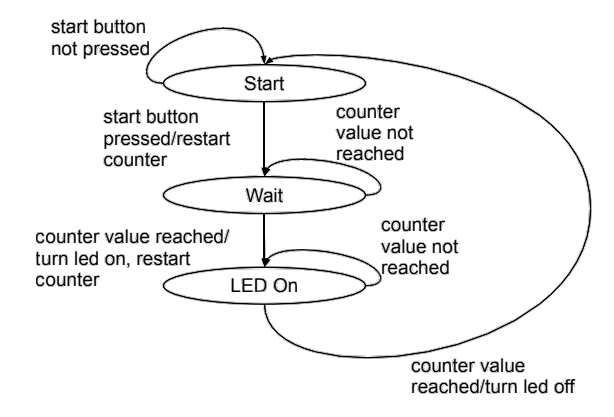
\includegraphics[width=0.5\linewidth]{images/FSM.png}

Figure \refstepcounter{figure}\arabic{figure}: Finite State Machine\label{fig:fsm}
\end{center}
\end{highlightblock}

\begin{highlightblock}[To-Do-List]
\begin{itemize}
\item Write the entities and architectures of the counter and FSM in VHDL.
	Use one .vhd file for each entity and one .vhd file for each architecture.
\item Write a testbench in VHDL (extra file). Simulate the system using Modelsim
	and hand in screenshots showing the output of the waveform window.
\item Discuss the results of the simulation in a few sentences.
\item Is the used finite-state-machine a Mealy or Moore machine? 
\end{itemize}
\end{highlightblock}
